\section{Problemas}

\begin{problem}[Sugerido para II o III nivel]
    En base a la siguiente figura.
    \begin{figure}[H]
        \centering
        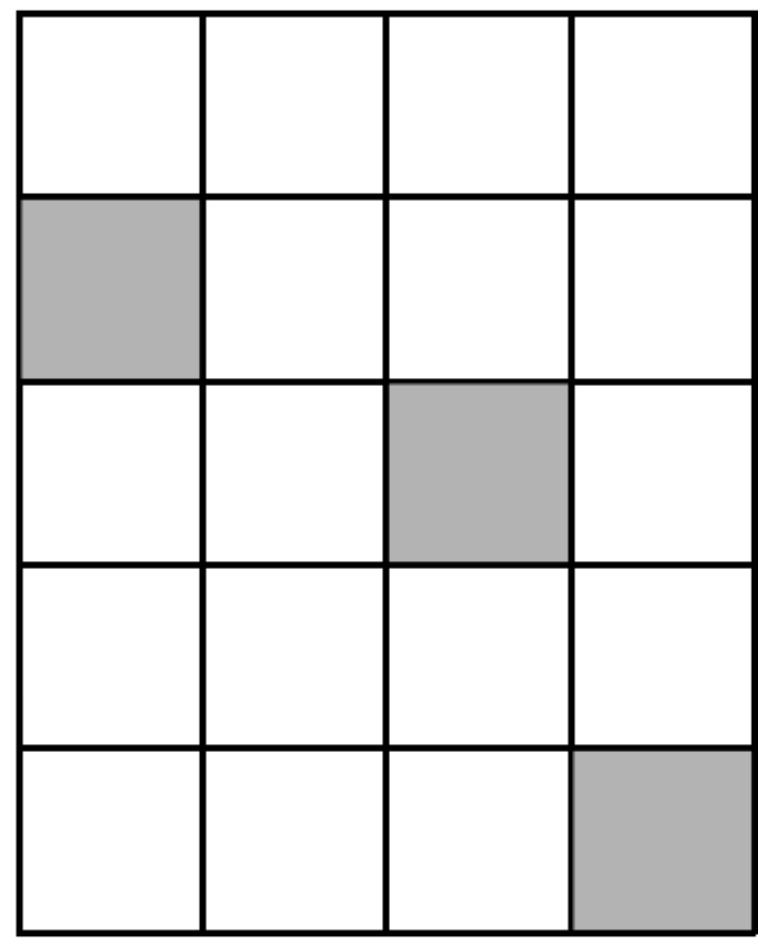
\includegraphics[width=3cm]{content/figure1}
    \end{figure}
    ¿Cuál es la cantidad mínima de cuadritos adicionales que deben pintarse para tener dos ejes de simetría en la figura?
\end{problem}

\begin{problem}[Sugerido para III o IV nivel]
    Un niño llamado Tato al aprender matemáticas inventó la operación numeral ($\#$), cuyo resultado es la suma de dos números dividida entre su resta.
    Por ejemplo, $9\ \#\ 3 = \frac{9 + 3}{9 - 3} = \frac{12}{6} = 2$.
    Hallar $(1\ \#\ 2025)\ \#\ 1$.
\end{problem}

\begin{problem}[Sugerido para IV nivel]
    Si $x^2 - 2x + 11$ se hace cero cuando $x = n$, entonces, sin hallar $n$, calcular el valor numérico de
    \[
        \frac{n^3 + 7n + 2047}{2}.
    \]
\end{problem}

\begin{problem}[Sugerido para IV nivel]
    En la figura, se tiene que $AB = AC = 40$ y $BC = 60$, donde $D$ es un punto medio de $BC$ y $M$ es punto medio de $AD$.
    Si se traza una cuerda $PQ$ paralela a $BC$ que pasa por $M$, hallar la longitud de $PQ$.
    \begin{figure}[H]
        \centering
        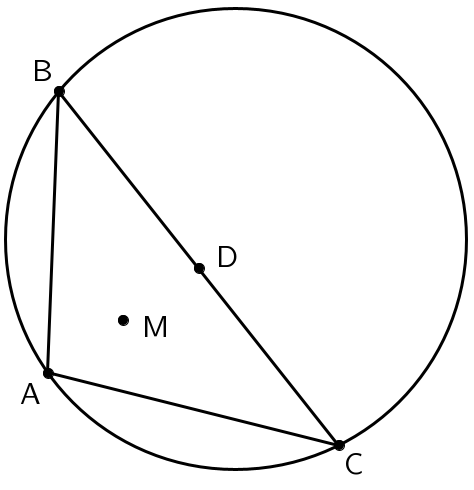
\includegraphics[width=6cm]{content/figure2}
    \end{figure}
\end{problem}

\begin{problem}[Sugerido para IV nivel]
    Diego enumeró una por una las páginas de su cuaderno de matemáticas, comenzando desde la página 1 y terminando en la página 2025
    ¿cuántas veces escribió la cifra 2 al enumerar su cuaderno?
\end{problem}

\begin{problem}[Sugerido para IV o V nivel]
    Fabiana compró lápices y carpetas a 11 y 9 córdobas, respectivamente.
    Curiosamente, pagó la misma cantidad de dinero en lápices y en carpetas
    ¿Cuántos artículos compró, sabiendo que la cantidad es mayor a 80 y menor a 120 artículos?
\end{problem}

\begin{problem}[Sugerido para IV o V nivel]
    Naho tiene muchos amigos, tantos que no sabe la cantidad exacta.
    Si tuviera 2 amigos menos, la cantidad sería múltiplo de 3.
    Si tuviera 3 amigos menos, la cantidad sería múltiplo de 10.
    ¿Cuántos amigos tiene Naho si la cantidad de amigos es mayor a 60 y menor a 100?
\end{problem}

\begin{problem}[Sugerido para IV o V nivel]
    $R(k)$ es una máquina que recibe entradas enteras y produce salidas enteras positivas.
    Si se tiene que $R(-1)\cdot R(2) = 4$ y
    \[
        R(a)^2 = R(a - b)\cdot R(b)
    \]
    para $a,b$ enteros cualesquiera, hallar $R(k)$.
\end{problem}

\begin{problem}[Sugerido para IV o V nivel]
    Hallar $Q(x^2 + 7x + 10)$ en términos de $x$, sabiendo que $Q(x^2 + x - 2) = x^3 - 27$ se cumple para cualquier número $x$.
\end{problem}


\begin{problem}[Sugerido para IV o V nivel]
    Hallar todos los enteros $m,n$ tales que
    \[
        m^2 + mn + n^2 = m - 2n - 1.
    \]
\end{problem}

\begin{problem}[Sugerido para V nivel]
    Brisa Marina quiere pagarle una deuda a Gerald, si ella solo tiene monedas de 3 y 5 córdobas y la deuda es un
    monto entero mayor a 7 córdobas ¿es posible pagar la deuda sea cual sea el monto?
\end{problem}